\documentclass[11pt]{article}

\usepackage[a4paper,margin=23mm]{geometry}
\usepackage[T1]{fontenc}
\usepackage[utf8]{inputenc}
\usepackage{amsmath,amssymb,amsthm}
\usepackage{array}
\usepackage{booktabs}
\usepackage{enumitem}
\usepackage{longtable}
\usepackage{tabularx}
\usepackage{xcolor}
\usepackage{listings}
\usepackage{tikz}
\usetikzlibrary{arrows.meta,calc,decorations.pathreplacing,fit,positioning,
  shapes.geometric}
\usepackage[hidelinks]{hyperref}

\setlength{\parindent}{0pt}
\setlength{\parskip}{0.55em}
\setlist{leftmargin=*,nosep}
\emergencystretch=3em
\renewcommand{\arraystretch}{1.16}

\definecolor{codebg}{RGB}{247,247,247}
\definecolor{rulegrey}{RGB}{92,92,92}
\definecolor{causalblue}{RGB}{31,78,121}
\definecolor{evidencegreen}{RGB}{46,125,50}
\definecolor{warningred}{RGB}{176,48,48}
\definecolor{softblue}{RGB}{232,241,249}
\definecolor{softgreen}{RGB}{235,246,235}
\definecolor{softred}{RGB}{252,237,237}
\definecolor{softgrey}{RGB}{242,242,242}

\lstset{
  basicstyle=\ttfamily\small,
  backgroundcolor=\color{codebg},
  frame=single,
  rulecolor=\color{rulegrey},
  breaklines=true,
  columns=fullflexible,
  keepspaces=true,
  showstringspaces=false,
  aboveskip=0.7em,
  belowskip=0.7em
}

\tikzset{
  process/.style={draw=causalblue,rounded corners,thick,fill=softblue,
    align=center,inner sep=6pt},
  evidencebox/.style={draw=evidencegreen,rounded corners,thick,fill=softgreen,
    align=center,inner sep=6pt},
  warningbox/.style={draw=warningred,rounded corners,thick,fill=softred,
    align=center,inner sep=6pt},
  neutralbox/.style={draw=rulegrey,rounded corners,thick,fill=softgrey,
    align=center,inner sep=6pt},
  flow/.style={-{Latex[length=2.4mm]},very thick,draw=causalblue},
  smalllabel/.style={font=\small,align=center}
}

\DeclareRobustCommand{\code}[1]{\texttt{\detokenize{#1}}}
\newcommand{\ABALearn}{\textsc{ABALearn}}
\newcommand{\Epos}{E^{+}}
\newcommand{\Eneg}{E^{-}}

\newtheorem{lemma}{Lemma}
\newtheorem{proposition}[lemma]{Proposition}
\newtheorem{corollary}[lemma]{Corollary}

\title{Finding 4: the folding-token ceiling is a restart ladder,\\[0.3em]
and under the target-wise encoding it is never binding\\[0.4em]
\large M1.3 Bucket 3 (M13-C3) --- evidence and reading}
\author{Working research synthesis}
\date{4 August 2026}

\begin{document}
\maketitle

\begin{center}
\fbox{\begin{minipage}{0.94\textwidth}
\textbf{Status.} Evidence record and bounded reading. \textbf{Not} a locked
Bucket~3 claim. All learner outputs cited here are pre-existing H4/H6/H7b
artefacts; this document adds a trace-level audit of those artefacts
(\path{band_replay_audit.py}) and no new learner runs.
\end{minipage}}
\end{center}

\section{The finding}

\begin{center}
\fbox{\begin{minipage}{0.94\textwidth}
\textbf{(a) Mechanism.} \code{folding_steps(M)} does not bound the number of
folds a run performs. It bounds a \emph{restart ladder}: nd learning starts at
\code{tokens(1)}, and whenever the entire search at allowance $T$ is exhausted
without a solution, \code{genT/6} sets $T\!+\!1$ and restarts the whole search,
while $T\!+\!1 \le M$.

\smallskip
\textbf{(b) Saturation.} Under the target-wise exact-value encoding, every
folding call terminates after \emph{exactly one} folding step, leaving $T-1$
tokens unspent. The allowance is therefore never binding, and a restart at a
higher allowance re-executes an identical search.

\smallskip
\textbf{(c) Consequence.} The ladder is a strict dichotomy. If a target is
solved, it is solved inside band~1 and $M$ has no effect whatsoever. If it is
not, the run performs exactly $M$ copies of one exhausted search: cost is affine
in $M$ and the outcome cannot change.

\smallskip
\textbf{(d) Measured.} On the H0 roots, trace length is \emph{exactly} affine in
$M$ with zero residual at $M\in\{1,2,5,10\}$, and bands $1,\dots,M$ are
byte-identical after normalising generated assumption indices, Prolog variable
numbers, and the printed token counter. At the inherited default $M=10$ this
costs $10.5\times$ and $9.8\times$ the wall-clock of $M=1$ for the two roots,
for a provably identical result.
\end{minipage}}
\end{center}

This is a statement about the learner, not about the collider fixture. Parts
(a) and (b) are read off \path{gen.pl}, \path{folding.pl},
\path{rote_learning.pl} and the generated \path{bk.aba}; part (c) follows; part
(d) is the H6a measurement, plus an audit over all $41$ nd cells produced in
this investigation.

\section{What \code{folding_steps} actually controls}

Two separate mechanisms carry the token count, and conflating them is what makes
the parameter look like a fold counter.

\paragraph{Inner: the allowance bounds folding steps within one call.}
\code{tokens(T)} is a dynamic fact initialised to $1$ in \path{folding.pl}. It is
read once per \code{folding/3} call and threaded as a countdown through
\code{fold_nd_wtc/7}, which consumes one unit per folding step:

\begin{lstlisting}
% folding.pl -- one token per folding step, then DONE or FAIL
fold_nd_wtc(C,_,_,Fs,[], Fs,C) :-
  C>=0,
  write(' '), write(C), write(': DONE'), nl.
fold_nd_wtc(C,Rs,H,FsI,[T|Ts], FsO,Co) :-
  C>=1,
  select_rule(Rs,T,R1),
  rule_hd(R1,I), rule_hd(R1,F), rule_bd(R1,[T|As]),
  write(' '), write(C), write(': folding '), show_term([T|Ts]), ...
  match(As,Ts,Asms, _,NewTs,ResTs),
  append(ResTs,NewTs, Ts1),
  C1 is C-1,
  fold_nd_wtc(C1,Rs,H,[F|FsI],Ts1, FsO,Co).
fold_nd_wtc(C,_,_,_,[T|Ts], _,C) :-
  C==0,
  write(' '), write(C), write(': FAIL - No more folding tokens left for '), ...
\end{lstlisting}

The trace is therefore self-documenting. A call that started with allowance $T$
and consumed $k$ tokens prints \code{T: folding} $\dots$ down to
\code{T-k+1: folding}, then \code{T-k: DONE}. A call that ran out prints
\code{0: FAIL - No more folding tokens left}.

\paragraph{Outer: $M$ bounds how many times the search is restarted.}
\code{genT/6} has two clauses. The first runs the search. The second fires only
when the first has failed \emph{completely} --- that is, when every folding
choice, assumption reuse and assumption introduction reachable at the current
allowance has been tried and refuted:

\begin{lstlisting}
% gen.pl -- the restart ladder
genT(R2,Ep0,En0,Ep,En, Ro) :-
  gen1(R2,Ep0,En0,Ep,En, Ro).
genT(R2,Ep0,En0,Ep,En, Ro) :-
  lopt(folding_mode(nd)),
  retract(tokens(T)),
  T1 is T+1,
  lopt(folding_steps(M)),
  ( T1 > M -> fail ; true ),
  nl, write('* Increasing folding tokens to: '), write(T1), nl,
  assert(tokens(T1)),
  genT(R2,Ep0,En0,Ep,En, Ro).
\end{lstlisting}

The recursive call re-enters \code{genT} with the \emph{same} $R2$, $\Epos$ and
$\Eneg$. Nothing is carried over from the failed attempt except the global fresh
name counter \code{current_new_pred/1}, which is why each band re-mints the same
assumptions under higher indices. That side effect is a useful witness: it makes
the restart visible in the trace.

\begin{figure}[ht]
\centering
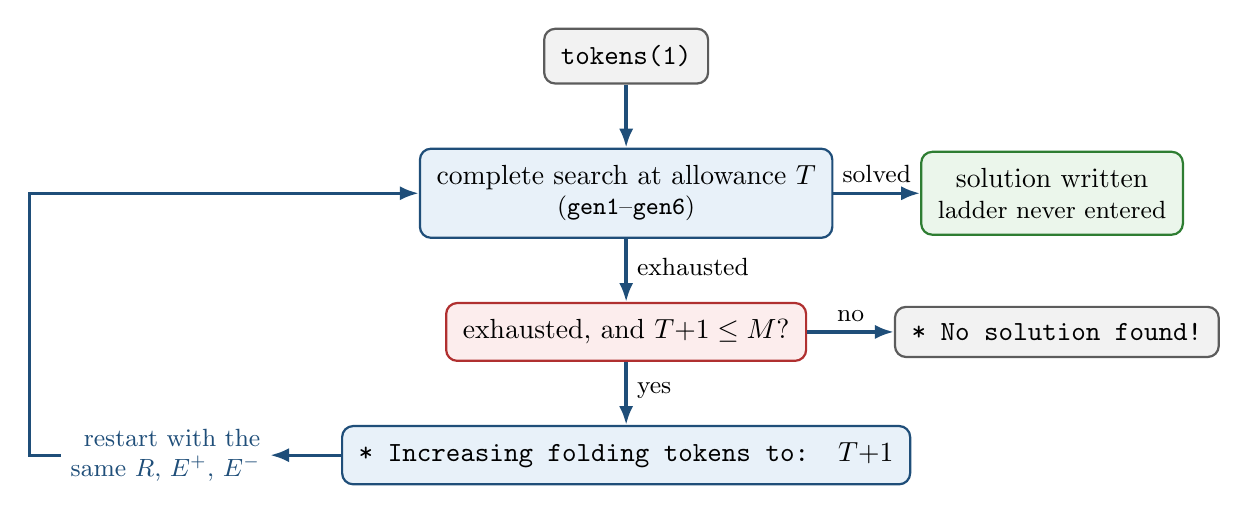
\begin{tikzpicture}[node distance=8mm and 11mm]
  \node[neutralbox] (init) {\code{tokens(1)}};
  \node[process,below=of init] (search)
    {complete search at allowance $T$\\[-1pt]\small(\code{gen1}--\code{gen6})};
  \node[warningbox,below=of search] (gate)
    {exhausted, and $T{+}1 \le M$?};
  \node[process,below=of gate] (inc)
    {\code{* Increasing folding tokens to: }$T{+}1$};
  \node[evidencebox,right=of search] (sol)
    {solution written\\[-1pt]\small ladder never entered};
  \node[neutralbox,right=of gate] (stop) {\code{* No solution found!}};
  \node[smalllabel,left=9mm of inc,align=right,text=causalblue] (lab)
    {restart with the\\same $R$, $\Epos$, $\Eneg$};
  \draw[flow] (init) -- (search);
  \draw[flow] (search) -- node[right,smalllabel,pos=0.45] {exhausted} (gate);
  \draw[flow] (search) -- node[above,smalllabel] {solved} (sol);
  \draw[flow] (gate) -- node[above,smalllabel] {no} (stop);
  \draw[flow] (gate) -- node[right,smalllabel,pos=0.45] {yes} (inc);
  \draw[flow] (inc.west) -- (lab.east);
  \draw[flow] (lab.west) -- ++(-4mm,0) |- (search.west);
\end{tikzpicture}
\caption{The two-level control. \code{tokens(T)} bounds folding steps inside one
call; $M$ bounds only how many times the outer loop restarts, and that loop is
entered only after a \emph{complete} failure. Everything a restart does is
therefore a repetition of work already refuted, except for whatever genuinely
new folds a larger allowance unlocks.}
\label{fig:two-level}
\end{figure}

\section{Why the allowance is never binding here}

The loop in Figure~\ref{fig:two-level} is only useful if a larger allowance
unlocks folds that a smaller one could not reach. That requires some folding
call to have run out of tokens. Under the target-wise encoding, none can.

\begin{proposition}[single-step folding]
\label{prop:single}
In the target-wise binary exact-value encoding, every rule offered to nd folding
has a body consisting of exactly one row-identifier equality, and every
background rule has a body consisting of exactly one row-identifier equality.
Consequently one folding step empties the to-be-folded list, and every
\code{folding/3} call consumes exactly one token.
\end{proposition}

The two halves are read directly off the artefacts. Rote learning emits
body-free facts, which \code{new_rule/3} normalises into a single equality:
\code{e_rote_learn(E, R) :- new_rule(E,[], R)}, printed as
\code{ert: a(A) <- [A=1]}. The generated background knowledge contains nothing
else either --- \path{input/bk.aba} for target $a$ consists solely of rules of
the form

\begin{lstlisting}
b_val_1(A) :- A=1.
b_val_0(A) :- A=8.
c_val_0(A) :- A=8.
\end{lstlisting}

and contains no rule body with two atoms. So in the recursive clause of
\code{fold_nd_wtc/7} the selected rule contributes \code{As = []}, hence
\code{match([],Ts,...)} returns \code{NewTs = []} and \code{ResTs = Ts}, which is
already \code{[]} for a single-equality body. The next call takes the
\code{DONE} clause. The continuation predicate \code{fold_nd_aux/5} cannot
re-enter folding either: its non-trivial clause needs \code{nselect/4}, which
requires a folded list of at least two elements.

\begin{lemma}[saturation implies replay]
\label{lem:replay}
If a complete search at allowance $T$ fails and no folding call printed
\code{FAIL - No more folding tokens left}, then the search at allowance $T+1$
explores the same folding results and fails identically.
\end{lemma}

\begin{proof}[Reason]
The counter is read only by \code{fold_nd_wtc/7}, where it appears in the guard
\code{C>=1} of the recursive clause and the guard \code{C==0} of the failure
clause. Raising the initial value only raises the depth at which those guards
bite. If no branch reached the failure clause, every branch terminated through
the counter-independent \code{DONE} clause, so the set of folding results is
unchanged; the rest of \code{gen1}--\code{gen6} is a deterministic function of
those results and of $\Epos,\Eneg$.
\end{proof}

\begin{corollary}
\label{cor:dichotomy}
Under Proposition~\ref{prop:single}, for every target either the search succeeds
in band~$1$, in which case \code{folding_steps} is inert, or it fails and the
run executes exactly $M$ identical bands before reporting
\code{completed_no_solution}.
\end{corollary}

Lemma~\ref{lem:replay} is stated in terms of the printed \code{FAIL} diagnostic
on purpose: that makes the hypothesis checkable in any run, including runs under
encodings for which Proposition~\ref{prop:single} does not hold. This is what
turns the finding into a usable test rather than a fact about one fixture
(Section~\ref{sec:implication}).

\section{Evidence}

\subsection{E1 --- the cost is exactly affine in $M$, and nothing else moves}

H6a varies only \code{folding_steps} on the frozen H0 table. The four
configurations are identical apart from $M$, and the learner-visible
\path{bk.aba}, \path{examples.json} and \path{data.csv} are identical per target
across all four.

\begin{center}
\small
\begin{tabular}{rlrrrrrr}
\toprule
$M$ & target & outcome & runtime (s) & trace lines & bands & NEW $\alpha$ & KO \\
\midrule
1  & $a$ & \code{completed_no_solution} & 6.638  & 549  & 1  & 9  & 16  \\
2  & $a$ & \code{completed_no_solution} & 13.117 & 1047 & 2  & 18 & 32  \\
5  & $a$ & \code{completed_no_solution} & 32.775 & 2541 & 5  & 45 & 80  \\
10 & $a$ & \code{completed_no_solution} & 69.952 & 5031 & 10 & 90 & 160 \\
\addlinespace
1  & $b$ & \code{completed_no_solution} & 6.797  & 555  & 1  & 9  & 16  \\
2  & $b$ & \code{completed_no_solution} & 13.487 & 1062 & 2  & 18 & 32  \\
5  & $b$ & \code{completed_no_solution} & 32.825 & 2583 & 5  & 45 & 80  \\
10 & $b$ & \code{completed_no_solution} & 66.473 & 5118 & 10 & 90 & 160 \\
\addlinespace
1,2,5,10 & $c$ & \code{solved} & 1.271--1.304 & 134 & 1 & 1 & 1 \\
\bottomrule
\end{tabular}
\end{center}

Every per-band quantity is constant, so every total is affine in $M$ with no
fitted slack:

\[
  \mathrm{lines}_a(M) = 51 + 498\,M, \qquad
  \mathrm{lines}_b(M) = 48 + 507\,M,
\]
\[
  \mathrm{NEW}(M) = 9\,M, \qquad \mathrm{KO}(M) = 16\,M, \qquad
  \text{token increases} = M-1 .
\]

Both line formulae reproduce all four measurements exactly. The constants are
the one-off option/rote-learning preamble ($50$ lines for $a$, $47$ for $b$) plus
the terminal \code{* No solution found!} line.

\begin{figure}[ht]
\centering
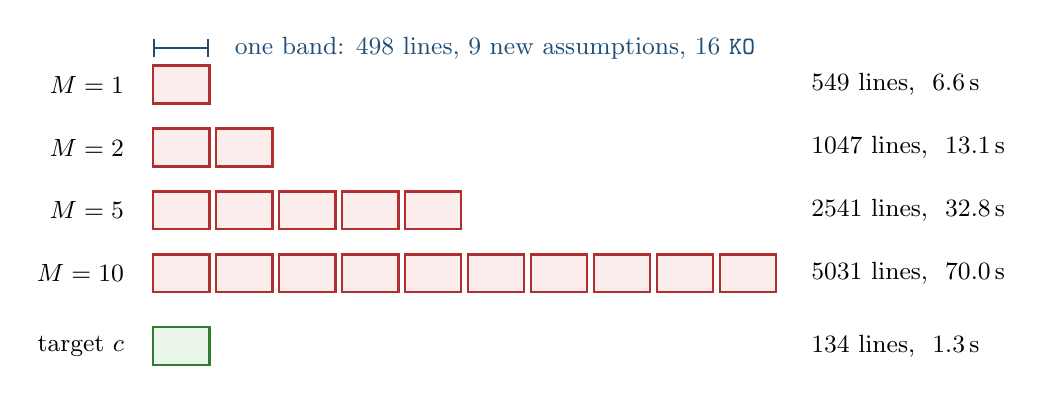
\begin{tikzpicture}[x=8mm,y=8mm]
  \foreach \m/\row/\lines/\secs in {1/0/549/6.6, 2/-1/1047/13.1,
                                    5/-2/2541/32.8, 10/-3/5031/70.0} {
    \node[smalllabel,anchor=east] at (-0.3,\row) {$M=\m$};
    \foreach \k in {1,...,\m}
      \draw[fill=softred,draw=warningred,thick]
        (\k-1,\row-0.30) rectangle (\k-0.10,\row+0.30);
    \node[smalllabel,anchor=west] at (10.3,\row) {\lines\ lines,\ \ \secs\,s};
  }
  \node[smalllabel,anchor=east] at (-0.3,-4.15) {target $c$};
  \draw[fill=softgreen,draw=evidencegreen,thick]
    (0,-4.45) rectangle (0.90,-3.85);
  \node[smalllabel,anchor=west] at (10.3,-4.15) {134 lines,\ \ 1.3\,s};
  \draw[|-|,thick,draw=causalblue] (0,0.58) -- (0.90,0.58);
  \node[smalllabel,anchor=west,text=causalblue] at (1.15,0.58)
    {one band: 498 lines, 9 new assumptions, 16 \code{KO}};
\end{tikzpicture}
\caption{H6a for target $a$, drawn as what the trace actually contains. Each red
block is one complete exhausted search, and all blocks in a row have the same
normalised hash; raising $M$ appends copies rather than extending a derivation,
which is why the totals are exactly affine and every row ends in
\code{completed_no_solution}. The solved child $c$ (green) occupies one block at
every $M$ because it never reaches the ladder.}
\label{fig:affine}
\end{figure}

\subsection{E2 --- the bands are the same search, not merely the same size}

Splitting each root trace at the \code{* Increasing folding tokens to:} lines and
hashing each band after normalising the three things that \emph{must} differ
between restarts --- generated assumption indices \code{alpha_N}, Prolog internal
variable numbers, and the printed token counter --- gives one hash for the whole
ladder.

\begin{center}
\small
\begin{tabular}{llrr}
\toprule
Trace (H0, $n{=}30$, $M{=}10$) & band lengths & bands & distinct hashes \\
\midrule
\code{baseline_cautious} target $a$ &
$50{+}498$, $498^{\times 8}$, $498{+}1$ & 10 & 1 \\
\code{baseline_cautious} target $b$ &
$47{+}507$, $507^{\times 8}$, $507{+}1$ & 10 & 1 \\
\bottomrule
\end{tabular}
\end{center}

The two extra terms are the only asymmetries: band~1 carries the one-off option
and rote-learning preamble, and the last band carries the terminal
\code{* No solution found!} line. Every band \emph{body} hashes the same.

Before normalisation the only residual differences between two interior bands are
Prolog variable numbers, e.g.

\begin{lstlisting}
band 2, line  555:  2: folding [A=1] with b_val_1(_7934): b_val_1(A) <- [A=1]
band 3, line 1053:  3: folding [A=1] with b_val_1(_7894): b_val_1(A) <- [A=1]
\end{lstlisting}

and bands $3$ through $9$ are identical even in those. The token counters
printed at each fold are exactly \code{folding@}$T$ followed by
\code{DONE@}$T{-}1$ in every band, at every $M$, for every target: one token
consumed, $T-1$ unspent. This is Proposition~\ref{prop:single} visible in the
trace, and it is the reason the bands coincide.

\subsection{E3 --- the solved control is untouched by the parameter}

Child $c$ solves inside band~1 at all four budgets, with a $134$-line trace, a
runtime of $1.27$--$1.30$\,s, and a \path{delta.aba} that is byte-identical
across all four collections:

\begin{lstlisting}
sha256  f9f75b60631b2a2aaac951521823e073bbfd5c73bd7aa96d259ca45cd426865a

c(A) :- alpha_1(A), a_val_1(A).
c_alpha_1(A) :- b_val_0(A).
assumption(alpha_1(A)).
contrary(alpha_1(A),c_alpha_1(A)) :- assumption(alpha_1(A)).
\end{lstlisting}

This is the first half of Corollary~\ref{cor:dichotomy} realised: a successful
run exits through the first \code{genT} clause and never reads
\code{folding_steps} at all. It also rules out the obvious alternative
explanation for E1 --- that larger $M$ inflates traces generally --- since the
same parameter change on the same table leaves this cell bit-for-bit unchanged.

\subsection{E4 --- the same ladder under a different assumption policy}

The H7b arm \code{nd_cautious_sechk} differs from \code{baseline_cautious} only
in \code{asm_intro(sechk)} instead of \code{relto}. It is a genuinely different
search: $74$ folding calls per band instead of $30$, $2.7\times$ the band length
and $2.4\times$ the runtime. The ladder structure is nevertheless identical.

\begin{center}
\small
\begin{tabular}{llrrrl}
\toprule
Arm ($M{=}10$) & target & runtime (s) & trace lines & bands & band body \\
\midrule
\code{baseline_cautious} (\code{relto}) & $a$ & 69.952  & 5031  & 10 & 498 lines, all identical \\
\code{nd_cautious_sechk} (\code{sechk}) & $a$ & 167.617 & 13731 & 10 & 1368 lines, all identical \\
\code{baseline_cautious} (\code{relto}) & $b$ & 66.473  & 5118  & 10 & 507 lines, all identical \\
\code{nd_cautious_sechk} (\code{sechk}) & $b$ & 172.883 & 13818 & 10 & 1377 lines, all identical \\
\addlinespace
\code{nd_cautious_sechk} (\code{sechk}) & $c$ & 2.242   & 200   & 1  & solved in band 1 \\
\bottomrule
\end{tabular}
\end{center}

So the ladder cost is not a property of one assumption-introduction policy: it
multiplies whatever the per-band search happens to cost. Under \code{sechk} the
inherited $M=10$ spends roughly $150$\,s per root on provably redundant replay.

\subsection{E5 --- saturation holds in every nd run in the investigation}

Proposition~\ref{prop:single} is a claim about the encoding, so it should hold
outside H0. \path{band_replay_audit.py} checks it over every target-wise
\path{prolog.stdout} whose \emph{effective} options include
\code{folding_mode(nd)}: $41$ cells spanning three fixtures (including the
pre-pivot four-node diamond), seven nd bundles, brave and cautious semantics,
\code{relto} and \code{sechk}, and $n\in\{30,50,60,90\}$.

\begin{center}
\small
\begin{tabularx}{\textwidth}{Xr}
\toprule
Audited property over the $41$ nd cells & Count \\
\midrule
folding calls that consumed more than one token & 0 \\
\code{FAIL - No more folding tokens left} lines & 0 \\
to-be-folded lists with more than one atom & 0 \\
\code{solved} cells that entered the ladder (bands $>1$) & 0 \ \ (of 27 solved) \\
\code{completed_no_solution} cells that entered the ladder & 12 \ \ (of 14; the other 2 are $M{=}1$) \\
laddered cells whose interior bands are not identical after normalisation & 0 \\
\bottomrule
\end{tabularx}
\end{center}

Two rows carry most of the generality. Zero token-exhaustion failures means the
hypothesis of Lemma~\ref{lem:replay} has held in every nd run ever produced
here. Zero solved cells with more than one band means no solution in this
investigation has ever depended on a second folding token --- so on the present
evidence \code{folding_steps(1)} would have produced every solution that
\code{folding_steps(10)} produced, at a tenth of the cost on the failures.

\section{Why the extra bands could not have helped}

Corollary~\ref{cor:dichotomy} explains why the replays are identical, but not why
band~1 fails. Those are different questions, and keeping them apart is what
stops Finding~4 from being read as evidence about root learnability.

Band~1 is a \emph{complete} refutation at allowance~$1$: for target $a$ it mints
$9$ assumptions and records $16$ \code{KO} verdicts before exhausting its
choices, including the decisive cautious refusal of the residual reuse that the
brave arm accepts,

\begin{lstlisting}
folding result: c_alpha_3(A) <- [b_val_0(A)]
 found: alpha_2/1 ... KO, cannot introduce an assumption for [b_val_0(A)]
\end{lstlisting}

The obstruction behind that verdict lives in $\langle\Epos,\Eneg\rangle$, not in
the fold: rows $9$ and $26$ present identical predictor literals with opposite
target labels, so no body over $b,c$ value predicates separates them at any
depth. That analysis belongs to Finding~3 and is not re-argued here. The point
for Finding~4 is only this: the ladder raises fold depth, the obstruction is not
fold depth, and \ABALearn{} has no mechanism for noticing the difference. It
spends its largest search budgets precisely where extra depth is irrelevant.

\begin{figure}[ht]
\centering
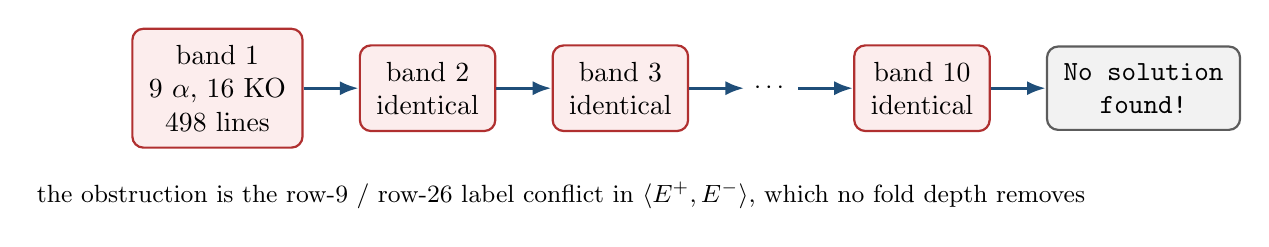
\begin{tikzpicture}[node distance=6mm and 7mm]
  \node[warningbox] (b1) {band 1\\9 $\alpha$, 16 KO\\498 lines};
  \node[warningbox,right=of b1] (b2) {band 2\\identical};
  \node[warningbox,right=of b2] (b3) {band 3\\identical};
  \node[smalllabel,right=of b3] (dots) {$\cdots$};
  \node[warningbox,right=of dots] (b10) {band 10\\identical};
  \node[neutralbox,right=of b10] (out) {\code{No solution}\\\code{found!}};
  \draw[flow] (b1) -- (b2); \draw[flow] (b2) -- (b3);
  \draw[flow] (b3) -- (dots); \draw[flow] (dots) -- (b10);
  \draw[flow] (b10) -- (out);
  \node[smalllabel,anchor=north] at
    ($(b1.south west)!0.5!(b10.south east)+(0,-4mm)$)
    {the obstruction is the row-9 / row-26 label conflict in
     $\langle\Epos,\Eneg\rangle$, which no fold depth removes};
\end{tikzpicture}
\caption{At $M=10$ the run pays ten complete refutations of the same
information-level conflict. The budget parameter and the reason for failure are
about different things.}
\label{fig:bands}
\end{figure}

\section{Design implication}
\label{sec:implication}

The useful consequence is not ``pick a smaller number''. It is that the ladder
already prints the information needed to decide whether continuing can possibly
help, so a \emph{sound} stopping test is available at no cost.

\begin{quote}
\textbf{Token-saturation test.} On a complete failure at allowance $T$, continue
to $T+1$ only if some folding call exhausted its allowance. Otherwise stop:
by Lemma~\ref{lem:replay} the next band is the same search.
\end{quote}

This differs in kind from a heuristic budget or a novelty detector. It does not
guess; it checks a condition under which the remaining work is provably
redundant. Three consequences follow for the present codebase.

\begin{enumerate}
  \item \textbf{For the current encoding the test always fires at $T=1$.} By
  Proposition~\ref{prop:single}, an allowance of one suffices for every
  target-wise cell in scope. The inherited ceiling of ten --- which
  comes from \path{configs/ecai2024_config.pl} and was copied unchanged into the
  \code{baseline_cautious}, \code{nd_brave_sechk} and \code{nd_cautious_sechk}
  configurations --- multiplies the cost of every unsolved nd target by ten for
  no possible gain. Measured: $69.95 \to 6.64$\,s and $66.47 \to 6.80$\,s on the
  two H0 roots.
  \item \textbf{The ladder is not useless in general.} It is useless exactly when
  the allowance is not binding. A background theory with multi-atom rule bodies
  would leave residual atoms to fold after the first step, the \code{FAIL}
  diagnostic would appear, and higher allowances would unlock genuinely new
  folds. So this finding constrains the \emph{encoding--parameter pairing}, not
  the parameter.
  \item \textbf{Search budget is the wrong lever for this failure mode.} On a
  target whose examples contain a predictor--label conflict, no folding budget
  helps. If unproductive search is to be avoided rather than merely truncated,
  the decision has to be made from the example set --- which is where a later
  Causal ABA layer could contribute, by supplying independent evidence about
  which predictor sets are worth attempting at all. That is a design hypothesis,
  not a result.
\end{enumerate}

\section{What is not established}

\begin{itemize}
  \item \textbf{Not a Bucket~3 claim.} The canonical hub records no approved
  claim, and this document does not create one.
  \item \textbf{Not a statement about all ABA Learning.} Proposition~\ref{prop:single}
  is contingent on the target-wise exact-value encoding, in which both rote rules
  and background rules have single-equality bodies. It says nothing about
  encodings with intensional or multi-atom background rules, where the allowance
  can bind.
  \item \textbf{Lemma~\ref{lem:replay} is argued from the control flow of
  \code{fold_nd_wtc/7}, not machine-checked.} Its empirical consequence --- band
  identity --- is verified on all $12$ laddered cells, which is corroboration,
  not proof.
  \item \textbf{$M=1$ sufficiency is verified, not proven, for solved cells.} All
  $27$ solved nd cells used one band, and the four H6a $c$ cells are
  byte-identical across $M$. The predicted $M=1$ behaviour of the
  \code{nd_cautious_sechk} roots has \emph{not} been run.
  \item \textbf{Runtime is affine only to within measurement noise.} Line counts
  are exactly affine; per-band runtime varies between $6.56$ and $7.00$\,s for
  target $a$, so the $M=10$ to $M=1$ ratio is $10.54$ rather than exactly $10$.
  \item \textbf{Root \code{completed_no_solution} is not mechanism recovery.}
  Roots $a$ and $b$ carry evaluator status
  \code{no_observed_parent_deterministic_rule}; the outcome is the absence of a
  cautiously acceptable covering theory, and Finding~4 is about the cost of
  establishing that absence, not about its correctness.
  \item \textbf{Single mechanism family.} Every fixture cited here has a
  deterministic AND child. Nothing in Sections~2--3 depends on the mechanism, but
  the measurements do not yet demonstrate that.
\end{itemize}

\section{Candidate reinforcement (not run; for discussion)}

Listed for the run-planning conversation, in decreasing value per unit of
compute. None of these has been executed.

\begin{enumerate}
  \item \textbf{Falsify or confirm the band prediction on a second search
  bundle.} Run \code{nd_cautious_sechk} at \code{folding_steps(1)} on the H0
  table. Prediction from E4: outcome unchanged, target-$a$ trace $= 1419$ lines
  equal to band~1 of the $M=10$ trace, runtime near $17$\,s. This is the cheapest
  test that could refute the finding.
  \item \textbf{Mirror the $M$ sweep on a different deterministic mechanism.}
  A binary fixture with stochastic roots and a non-AND deterministic child would
  show that the affine law and band identity do not depend on the mechanism, only
  on the encoding.
  \item \textbf{Exhibit a binding allowance.} A background theory containing one
  multi-atom rule should make the \code{FAIL - No more folding tokens left}
  diagnostic appear and make a higher allowance materially different. This would
  complete the dichotomy and show that the saturation test discriminates rather
  than always firing.
\end{enumerate}

\appendix

\section{Provenance and reproduction}

Fixture and sample: \path{causal/fixtures/specs/m13_bucket3_binary_collider_and.yaml};
frozen \path{samples/n30_seed42.csv}, with

\begin{lstlisting}
sha256  1edae465d0f6b6b662b3c4ed4863af21c1d9b0c1cf428774731dd3f43282a8ca
\end{lstlisting}

Learner collections, all under
\path{causal/outputs/aba_learning/targetwise/m13_bucket3_binary_collider_and/}:
\path{baseline_cautious_steps1}, \path{baseline_cautious_steps2},
\path{baseline_cautious_steps5}, \path{baseline_cautious} (the reused H4
steps-10 collection), and \path{nd_cautious_sechk}, each at \path{n30_seed42}.

The H6a collections were produced by (H6 record, not re-run for this document):

\begin{lstlisting}
python -m causal.targetwise.cli run \
  --config causal/configs/targetwise/m13_bucket3_binary_collider_and/baseline_cautious_steps1/n30_seed42.yaml
python -m causal.targetwise.cli run \
  --config causal/configs/targetwise/m13_bucket3_binary_collider_and/baseline_cautious_steps2/n30_seed42.yaml
python -m causal.targetwise.cli run \
  --config causal/configs/targetwise/m13_bucket3_binary_collider_and/baseline_cautious_steps5/n30_seed42.yaml
\end{lstlisting}

The trace audit reported in E2 and E5 is reproduced from the repository root by:

\begin{lstlisting}
python docs/experiments/qualitative/M13-C3-binary-collider-and/band_replay_audit.py
\end{lstlisting}

Engine files consulted read-only: \path{folding.pl} (\code{tokens/1},
\code{fold_nd_wtc/7}, \code{fold_nd_aux/5}), \path{gen.pl} (\code{genT/6},
\code{gen_new_name/1}), \path{rote_learning.pl} (\code{e_rote_learn/2}),
\path{asp_utils.pl} (\code{new_rule/3}).
Configurations: \path{configs/baseline_cautious_config.pl} and its
\code{steps1}/\code{steps2}/\code{steps5} variants,
\path{configs/nd_cautious_sechk_config.pl}, \path{configs/ecai2024_config.pl}.

Primary experiment records: \path{h6_folding_and_n_ablation.md} / \path{.tex}
(H6a/H6b), \path{h4_cautious_vs_brave.md} (the $M=10$ root cost being explained),
\path{h7b_cautious_relto_vs_sechk.md} (the \code{sechk} arm),
\path{experiment.md} (investigation hub).

\paragraph{Line-count convention.} ``Trace lines'' counts lines of text in
\path{output/prolog.stdout}, matching the figures tabulated in the H6 record.
Root traces have no terminating newline on their final line, so \code{wc -l}
reports one fewer for those cells; the audit script normalises this.

\end{document}
